\chapter{Implementation}
\label{implementation}

The \ac{ASTRID} project focuses on enabling drone control through voice commands powered by Large Language Models (\acp{LLM}). 
As part of the initiative, two Proofs of Concept (\acp{PoC}) were developed, each addressing a unique challenge in the application of \acp{LLM} for drone operations.

\section{Methodology: Drone Command Generation}
\subsection{Overview}
The first \ac{PoC} aimed to explore the potential of few-shot prompting to generate a sequence of precise drone commands based on natural language instructions. 
This methodology involved designing a set of adaptable prompts capable of handling varying levels of complexity in user inputs.

\subsection{Prompt Engineering}
Prompt engineering focused on defining clear parameters for movement and rotation. The drone commands followed predefined formats such as "Go Front", "Turn Left", "Go Right", and "Go Up", 
with the goal of translating user requests for movement into a chain of executable instructions. 
Key challenges included refining the prompts to ensure that the \ac{LLM} generated commands that were both accurate and feasible, given the constraints of the drone SDK.

For instance, a simple prompt like "Move forward 50 cm and then turn left 90 degrees" would result in a sequence of commands like:  
\texttt{Go Front, Go Front, Go Front, Go Front, Go Front, Turn Left, Turn Left, Turn Left}.  
This approach allowed the \ac{LLM} to handle both simple and more complex instructions, including geometric shapes and multi-step movements. 
For complex shapes like squares or circles, the prompt was adjusted to guide the \ac{LLM} step-by-step, ensuring that it could break down larger tasks into smaller, actionable commands.

\section{Methodology: Real-time Video Streaming}
\subsection{Overview}
The second \ac{PoC} focused on improving the latency of real-time video streaming from the drone. 
Prior to this work, the Innovations Team had relied on YouTube to stream drone footage, but this solution suffered from significant latency, often exceeding 10 seconds. 
To address this challenge, an NGINX \ac{RTMP} server was set up to directly receive the \ac{RTMP} stream from the drone, offering a significant improvement in latency.

\subsection{RTMP Server Configuration}
The implementation of the \ac{RTMP} server involved several key steps:
\begin{itemize}
    \item Configuring an NGINX server with the \ac{RTMP} module to accept and forward \ac{RTMP} streams.
    \item Setting up the server on a local machine (MacBook) and testing its performance with tools like \texttt{ffmpeg} to measure latency.
    \item Fine-tuning parameters to minimize delay and ensure smooth streaming.
\end{itemize}

\section{Implementation: Drone Command Generation}
\subsection{Few-shot Prompting in PyGame}
The first \ac{PoC} was implemented in a simulation environment using PyGame, where the \ac{LLM}-generated commands could be executed in real-time. 
The simulation employed the same command set as the drone SDK, including basic movement and rotation instructions. 
The prompts were designed to ensure that the \ac{LLM} could generate commands that were both feasible and precise, considering the drone's movement constraints.

The process involved sending user input to the \ac{LLM} via a chatbot interface, where the \ac{LLM} would respond with a series of commands. 
These commands were then executed in the simulation, with the drone moving or rotating based on the generated instructions. 
Prompt engineering was iteratively refined based on feedback from initial tests, ensuring that the \ac{LLM} understood the task and produced relevant commands.

This implementation enabled testing of complex scenarios, such as multiple turns or navigating specific shapes, and helped refine the \ac{LLM}'s response to these instructions.

\subsection{Prompt Engineering and Refinement}
Initially, the \ac{LLM} used for few-shot prompting was GPT-4o-mini, but it was quickly replaced by GPT-4o due to the former's inability to generate accurate drone commands. 
Additionally, system prompts were refined to ensure that the \ac{LLM} could produce precise and actionable instructions for drone movement and behavior. 
The final iteration of the system prompt, as shown in the code snippet \ref{lst:prompt_engineering}, ensured the required accuracy.

\subsection{PyGame Simulation: Visualization of a simple command}
To better understand the behavior of the simulated drone, a series of screenshots were taken during the execution of various commands. 
These images highlight the initial setup, the command interface, and the results of executing a single movement instruction.

\begin{figure}[H]
    \centering
    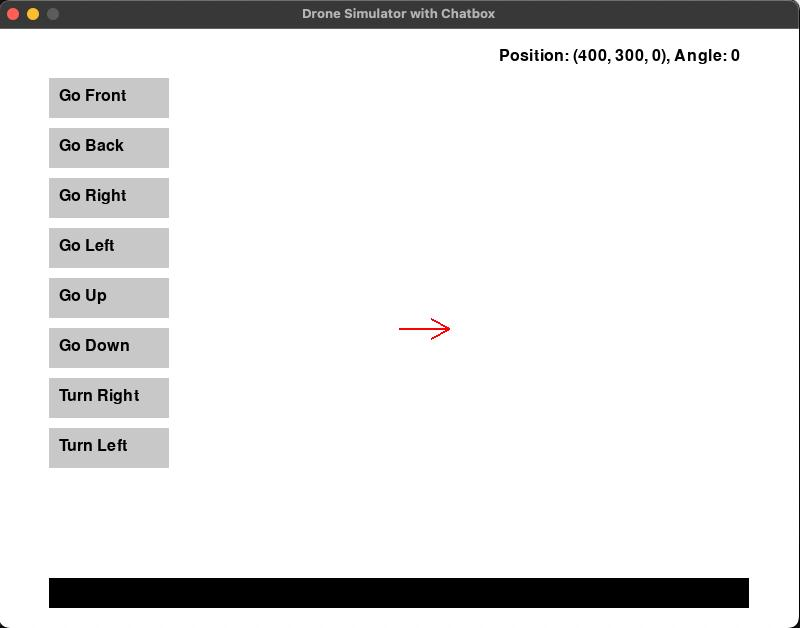
\includegraphics[width=0.6\textwidth]{img/sim_pos_start.jpeg}
    \caption{Initial position of the drone in the PyGame simulation. The drone is stationary, and no commands have been entered yet.}
    \label{fig:sim_pos_start}
\end{figure}

\begin{figure}[H]
    \centering
    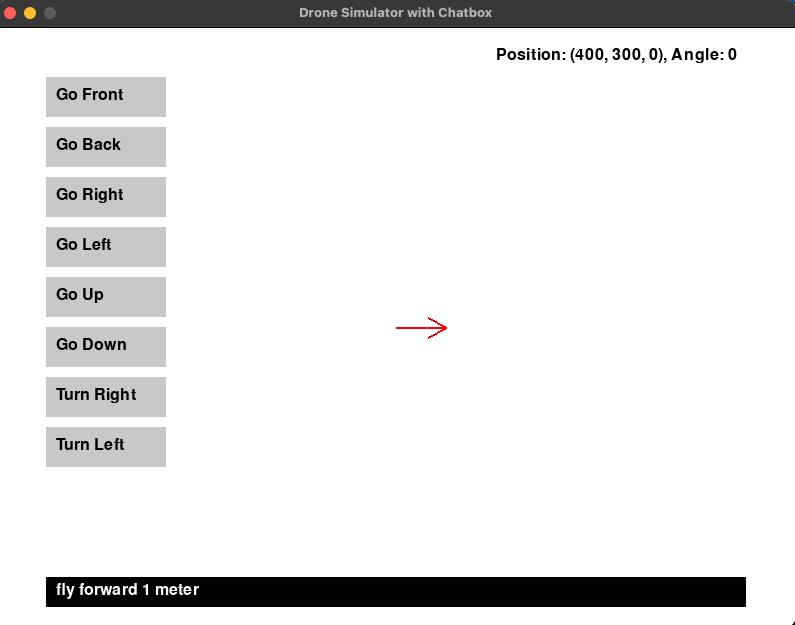
\includegraphics[width=0.6\textwidth]{img/sim_command_forward.jpeg}
    \caption{Chatbox interaction, the command ``fly forward 1 meter'' is entered}
    \label{fig:sim_command_forward}
\end{figure}

\begin{figure}[H]
    \centering
    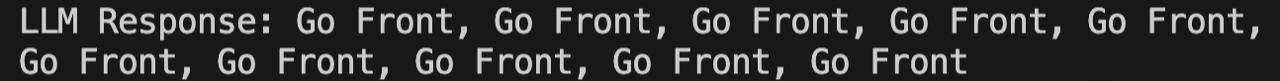
\includegraphics[width=0.7\textwidth]{img/response_forward.jpeg}
    \caption{\ac{LLM} response to the ``fly forward 1 meter'' command. The \ac{LLM} outputs a chain of 10 ``Go Front'' commands since each command moves the drone by 10 cm.}
    \label{fig:response_forward}
\end{figure}
\begin{figure}[H]
    \centering
    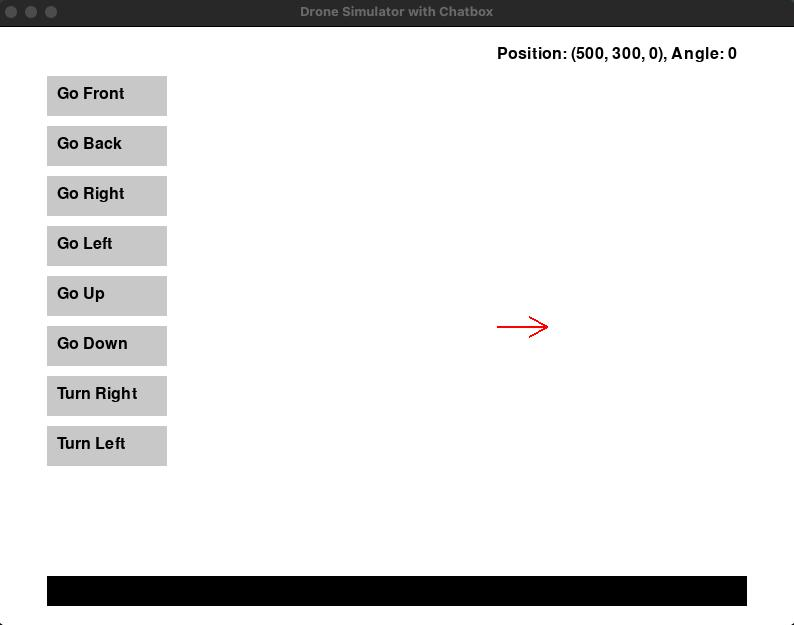
\includegraphics[width=0.6\textwidth]{img/sim_pos_forward.jpeg}
    \caption{Resulting position of the drone after executing the command chain. The drone has moved 1 meter forward.}
    \label{fig:sim_pos_forward}
\end{figure}

These visualizations demonstrate how the simulation progresses from an initial state to the execution of a movement command, 
providing insights into the \ac{LLM}'s effectiveness in generating actionable drone instructions.

\subsection{PyGame Simulation: Visualization of a Complex Command}
To further demonstrate the capabilities of the PyGame simulation with the latest iteration of the system prompt, a more complex command was executed: instructing the drone to fly in a circle with the radius 50 cm. 
This command was selected to test the system's ability to handle scenarios that go beyond simple chains of commands, such as chains of solely moving in a direction or turning, 
which are insufficient for real-world applications.

\begin{figure}[H]
    \centering
    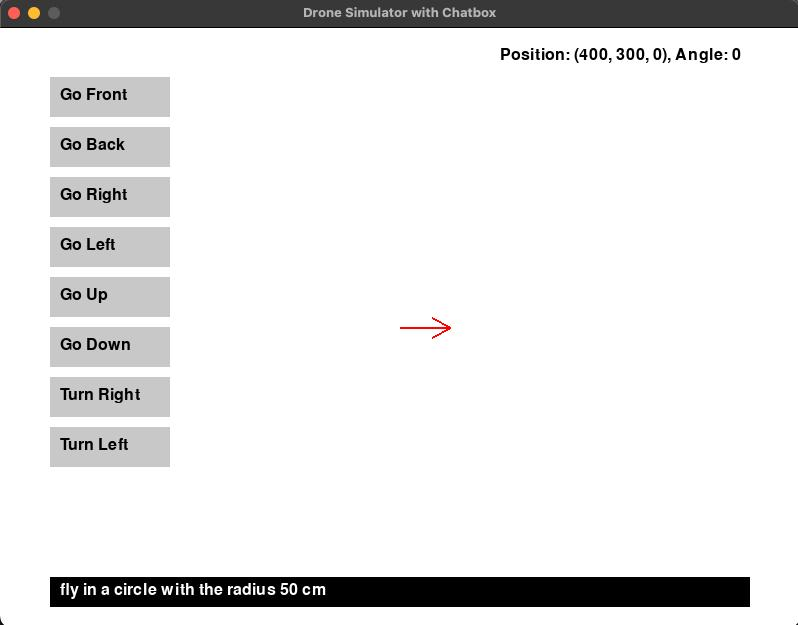
\includegraphics[width=0.6\textwidth]{img/sim_command_circle.jpeg}
    \caption{Chatbox interaction, the command ``fly in a circle with the radius 50 cm'' is entered.}
    \label{fig:sim_command_circle}
\end{figure}

\begin{figure}[H]
    \centering
    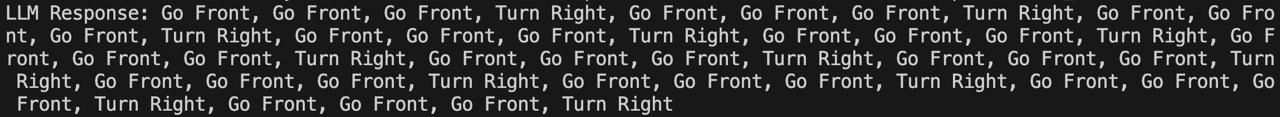
\includegraphics[width=0.9\textwidth]{img/response_circle.jpeg}
    \caption{\ac{LLM} response to the ``fly in a circle with the radius 50 cm'' command. The response contains a sequence of repeated ``Go Front'' and ``Turn Right'' commands to approximate a circular path.}
    \label{fig:response_circle}
\end{figure}

One part of the system prompt (\ref{lst:prompt_engineering}) includes instructions specifically tailored for generating a circle trajectory. As shown in the snippet (\ref{lst:circle_instructions}), 
these instructions guide the \ac{LLM} in calculating the necessary steps to approximate a circle of any size while adhering to the drone's operational constraints. 
These constraints include moving in 10 cm increments and turning in 30-degree steps, ensuring the generated commands are both feasible and precise.


\begin{lstlisting}[caption={Prompt Engineering Circle Instructions}, label={lst:circle_instructions}]
"Circle Instructions:\n"
"1. For a circle with radius n cm, calculate the circumference using the formula C = 2 * pi * n, where n is the radius.\n"
"2. The drone can only move forward in increments of 10 cm, so round the forward movement to the nearest 10 cm to fit the circumference.\n"
"3. Divide the circle into 12 equal segments of 30 degrees each (to complete 360 degrees). For each segment, move forward by a distance proportional to the radius.\n"
"4. The distance moved forward per segment can be calculated by dividing the circle's circumference by 12 (the number of 30-degree segments). Since the drone moves in 10 cm increments, round the distance to the nearest 10 cm.\n"
"   - For example, if the circumference is 628 cm, the drone moves approximately 52 cm per segment (rounded to the nearest 10 cm, which is 50 cm). This would mean the drone moves forward 5 times (10 cm each) in each 30-degree turn.\n"
"5. Repeat the movement and rotation steps 12 times to approximate the circle.\n"
"6. Example: For a circle with radius 100 cm (circumference = 628 cm), the drone would move forward 5 times (10 cm per step) for each of the 12 segments, turning right 30 degrees after each movement. The sequence of commands would look like this: 'Go Front, Go Front, Go Front, Go Front, Go Front, Turn Right, Go Front, Go Front, Go Front, Go Front, Go Front, Turn Right, ...' (repeat for 12 steps).\n"
\end{lstlisting}

\begin{figure}[H]
    \centering
    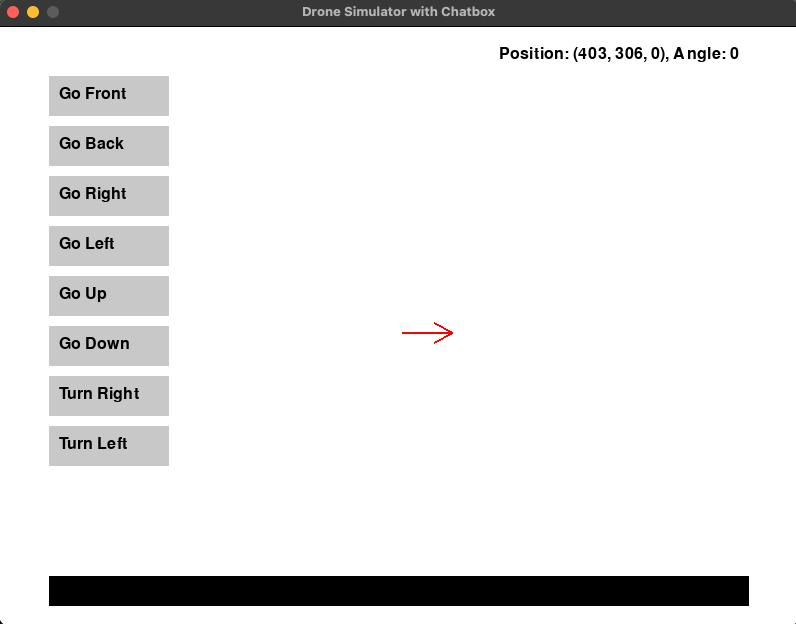
\includegraphics[width=0.6\textwidth]{img/sim_pos_circle.jpeg}
    \caption{Resulting position of the drone after executing the command sequence. Due to rounding, the drone ends up slightly off its starting position, 3 cm east and 6 cm north.}
    \label{fig:sim_pos_circle}
\end{figure}

The drone successfully completes the circle using the calculated steps, showcasing the \ac{LLM}'s ability to generate precise and actionable commands for complex tasks. 
While minor deviations occur due to rounding errors, the system prompt ensures that the \ac{LLM} produces commands that are both feasible and as accurate as possible within the constraints of the drone's movement capabilities. 
This demonstrates the robustness of the prompt engineering in enabling the \ac{LLM} to handle complex real-world scenarios.

\section{Implementation: Real-Time Video Streaming}
\subsection{NGINX RTMP Server for Video Streaming}
The second \ac{PoC} aimed to improve the real-time video streaming experience by reducing latency, transitioning from YouTube to a local NGINX \ac{RTMP} server. 
This solution was tested with the different encoding settings H.264 and H.265 but the results were inconclusive in determining which encoding performed better. 
However, a key configuration, \texttt{sync}, was crucial for ensuring stable streaming. After testing, it was found that a \texttt{sync} value of 5ms provided the best results, 
though further testing under varying conditions is recommended.

The setup process involved installing and configuring the NGINX \ac{RTMP} module on the MacBook, adjusting settings to handle the stream efficiently. 
Results showed that the \ac{RTMP} server reduced latency significantly, achieving a stream delay of approximately 1-2 seconds—substantially better than the previous YouTube-based solution.

Although this setup worked well in the test environment using a mobile hotspot, subsequent tests on SAP's Wi-Fi network were hindered by firewall issues. 
This could be resolved in a production environment by implementing a dedicated router or an alternative network configuration.

\section{Challenges and Limitations}
Several challenges were encountered during the implementation of both \acp{PoC}. For the few-shot prompting task, initial testing with GPT-4o-mini proved insufficient for generating accurate drone commands. 
Transitioning to GPT-4o was essential for achieving the desired results, as it offered improved comprehension and response accuracy. 
Additionally, the system prompts required several iterations to ensure the \ac{LLM} generated precise, actionable instructions for drone movement.

For the \ac{RTMP} streaming, the primary hurdle was the network setup. Although the mobile hotspot provided a temporary solution, a more stable network infrastructure is necessary for long-term deployment. 
Additionally, the tests to determine the best video settings were inconclusive, warranting further investigation to identify the optimal configuration.

Despite these challenges, 
both \acp{PoC} demonstrated the potential of using \acp{LLM} in drone control and highlighted the importance of real-time video streaming in applications such as surveillance and remote monitoring.
